\chapter{Hình học, thông tin và định luật diện tích của lỗ đen}

\lectureoverview{Điểm đến đã được báo trước là vũ trụ học, nhưng con đường ngắn nhất tới đó lại bắt đầu bằng việc quay về thuyết tương đối hẹp. Metric cho ta biết hình học của không-thời gian, còn điều kiện thời gian riêng bằng không cho ta biết ánh sáng truyền như thế nào. Chúng ta sẽ mang quy tắc duy nhất ấy vào hình học Schwarzschild, phân biệt chân trời với kỳ dị, rồi hỏi thông tin sẽ ra sao khi một lỗ đen bức xạ dần mất đi. Câu trả lời bắt đầu từ entropy thông thường và kết thúc ở lập luận một bit của Bekenstein: lỗ đen lưu trữ thông tin theo đơn vị diện tích chân trời chứ không phải thể tích.}

Susskind tạm gác ngắn gọn bản tổng kết đã hứa về những thành công và thất bại của lý thuyết dây. Ông nói đã muộn, và nội dung thực chất hữu ích hơn một cuộc kiểm kê. Nội dung thực chất tối nay là phần hình học và nhiệt động lực học tối thiểu cần để phát biểu bài toán thông tin của lỗ đen.

\section{Một quy tắc duy nhất cho ánh sáng}

Thuyết tương đối hẹp xem không gian và thời gian là một đối tượng hình học duy nhất. Với các biến cố lân cận cách nhau bởi \(dt,dx,dy,dz\), Susskind dùng quy ước chủ yếu dấu trừ và viết
\begin{equation}
d\tau^2=dt^2-\frac{1}{c^2}\left(dx^2+dy^2+dz^2\right).
\end{equation}
Dấu trái ngược nhau của phần thời gian và phần không gian phân biệt hình học Minkowski với hình học Euclid bốn chiều. Hệ số \(1/c^2\) chỉ đơn thuần điều hòa đơn vị; bằng cách đo thời gian và khoảng cách theo những đơn vị tương thích, ta có thể đặt \(c=1\).

Với khoảng tách kiểu thời gian \(d\tau^2>0\), và \(d\tau\) là thời gian riêng được một chiếc đồng hồ đi theo quỹ đạo ấy ghi lại. Trái lại, các khoảng tách kiểu không gian có \(d\tau^2<0\). Trường hợp cần cho tối nay nằm đúng giữa hai loại đó. Một tia sáng đi theo quỹ đạo \emph{null},
\begin{equation}
d\tau^2=0.
\end{equation}
Trước hết giới hạn vào chuyển động dọc theo trục \(x\) thì được
\begin{align}
0&=dt^2-\frac{dx^2}{c^2},\\
c\,dt&=\pm dx,\\
\frac{dx}{dt}&=\pm c.
\end{align}
Các dấu mô tả các tia đi sang phải và sang trái. Giá trị số gán cho \(c\) thay đổi khi thay xentimét bằng mét hay kilômét; mệnh đề bất biến không phải là một con số mà là điều kiện null.

Thuyết tương đối rộng làm metric phức tạp hơn, chứ không phải quy tắc này. Với các tọa độ \(x^\mu\), \(\mu=0,1,2,3\),
\begin{equation}
ds^2=g_{\mu\nu}(x)\,dx^\mu dx^\nu,
\end{equation}
trong đó các chỉ số lặp được lấy tổng và các hệ số có thể thay đổi từ điểm này sang điểm khác. Để tìm các hướng truyền ánh sáng được phép cục bộ, hãy cho dạng toàn phương này bằng không.

\section{Tọa độ cầu và metric Schwarzschild}

Một lỗ đen không quay có đối xứng cầu, vì vậy tọa độ Cartesian che khuất cấu trúc hữu ích. Hãy để \(r\) đo khoảng cách xuyên tâm và \(\theta,\phi\) xác định một hướng trên mặt cầu đơn vị. Phần tử độ dài của nó là
\begin{equation}
d\Omega^2=d\theta^2+\sin^2\theta\,d\phi^2.
\end{equation}
Vì thế, trên một mặt cầu bán kính \(r\), các độ dời góc đóng góp \(r^2d\Omega^2\). Không-thời gian phẳng trong tọa độ cầu là
\begin{equation}
d\tau^2=dt^2-\left(dr^2+r^2d\Omega^2\right),
\qquad (c=1).
\end{equation}

Susskind không suy ra nghiệm lỗ đen từ các phương trình Einstein. Ông viết nó ra và yêu cầu chúng ta xem xét nó. Bảng viết làm rõ sự so sánh được nhắm tới.

\begin{figure}[htbp]
\centering
\includegraphics[width=0.86\textwidth]{lecture_02_figure_02.png}
\caption{Không-thời gian phẳng trong tọa độ cầu nằm phía trên biến dạng Schwarzschild. Hệ số lặp lại \(1-2GM/(c^2r)=1-R_s/r\) và phác thảo theo phương bán kính được thấy cùng nhau.}
\lectureframe{00:19:12.520}
\end{figure}

Đối với một lỗ đen khối lượng \(M\), định nghĩa bán kính Schwarzschild
\begin{equation}
R_s=\frac{2GM}{c^2}.
\end{equation}
Phần tử độ dài bên ngoài là
\begin{equation}
d\tau^2=\left(1-\frac{R_s}{r}\right)dt^2
-\frac{dr^2/c^2}{1-R_s/r}
-\frac{r^2}{c^2}d\Omega^2.
\label{eq:schwarzschild-explicit-c}
\end{equation}
Tương đương, sau khi đặt \(c=1\),
\begin{equation}
ds^2=\left(1-\frac{2GM}{r}\right)dt^2
-\frac{dr^2}{1-2GM/r}-r^2d\Omega^2.
\label{eq:schwarzschild}
\end{equation}
Ở rất xa, \(R_s/r\ll1\), và metric phẳng trong tọa độ cầu lại xuất hiện. Phép kiểm tra tiệm cận này quan trọng hơn việc học thuộc công thức, dù Susskind khuyên nên làm điều sau như vốn liếng cho các buổi tiệc cocktail.

\editorialnote{Bảng viết luân phiên giữa \(d\tau^2\) và \(ds^2\) và không hiển thị nhất quán mọi hệ số của \(c\). Phương trình~\eqref{eq:schwarzschild-explicit-c} tuân theo quy ước tọa độ thời gian của bài giảng, trong đó \(t\) có đơn vị thời gian. Dạng chuẩn với \(x^0=ct\) là tương đương về mặt đại số.}

\subsection{Chân trời không phải là kỳ dị}

Có hai bán kính trông đáng ngờ trong các tọa độ này. Tại \(r=R_s=2GM\) trong đơn vị tự nhiên, hệ số của \(dt^2\) triệt tiêu còn hệ số của \(dr^2\) phân kỳ. Tại \(r=0\), bản thân độ cong trở nên kỳ dị. Đây không phải là hai phiên bản của cùng một sự kiện:
\begin{equation}
\begin{aligned}
r=R_s &:\quad \text{horizon},\\
r=0 &:\quad \text{curvature singularity}.
\end{aligned}
\end{equation}

Các lực thủy triều cho ta sự phân biệt vật lý. Trường hấp dẫn biến thiên trên một vật thể có kích thước: chân có thể bị kéo mạnh hơn đầu, làm vật thể bị kéo dài ra trong khi các phương ngang bị ép lại. Tại chân trời, các lực thủy triều ấy là hữu hạn, và tại chân trời của một lỗ đen đủ lớn chúng có thể rất nhỏ. Không nhất thiết có điều gì thảm khốc cục bộ xảy ra ở đó. Ngược lại, tại \(r=0\), các lực thủy triều phân kỳ. Những hệ số đáng báo động tại \(r=R_s\) báo hiệu một khuyết tật của tọa độ Schwarzschild; kỳ dị tại \(r=0\) mới là vật lý.

\editorialnote{Tính hữu hạn của độ cong tại \(r=R_s\) có thể được kiểm tra từ vô hướng Kretschmann \(R_{\mu\nu\rho\sigma}R^{\mu\nu\rho\sigma}=48G^2M^2/(c^4r^6)\), đại lượng này hữu hạn ở chân trời và chỉ phân kỳ khi \(r\to0\). Bất biến này không được viết ra trong bài giảng, nhưng nó làm cho sự phân biệt bằng lực thủy triều ở trên trở nên chính xác.}

\section{Ánh sáng theo phương bán kính gần chân trời}

Giờ hãy quay lại quy tắc duy nhất ấy. Một tia theo phương bán kính giữ cố định vị trí góc của nó, nên \(d\Omega=0\), và tia sáng có \(ds^2=0\). Trong đơn vị \(c=1\), Phương trình~\eqref{eq:schwarzschild} cho
\begin{equation}
0=\left(1-\frac{2GM}{r}\right)dt^2
-\frac{dr^2}{1-2GM/r}.
\end{equation}
Nhân với \(1-2GM/r\) rồi lấy căn bậc hai cho hai nhánh,
\begin{align}
dr&=\pm\left(1-\frac{2GM}{r}\right)dt,\\
\frac{dr}{dt}&=\pm\left(1-\frac{2GM}{r}\right).
\label{eq:radial-null}
\end{align}
Dấu cộng là tia đi ra và dấu trừ là tia đi vào. Ở rất xa, các tốc độ tọa độ của chúng tiến tới \(\pm1\). Tại chân trời, cả hai đều thỏa \(\lvert dr/dt\rvert\to0\): theo thời gian tọa độ Schwarzschild, một tia đi ra dường như đứng yên ở đó, còn một tia đi vào cần thời gian tọa độ vô hạn để tới nơi.

\begin{figure}[htbp]
\centering
\includegraphics[width=0.82\textwidth]{lecture_02_figure_03.png}
\caption{Bản phác thảo bảng đen \(t\)-\(r\) đã hoàn chỉnh: các tia null theo phương bán kính trở nên gần như thẳng đứng khi tiến tới chân trời nét đứt.}
\lectureframe{00:30:25.000}
\end{figure}

\begin{figure}[htbp]
\centering
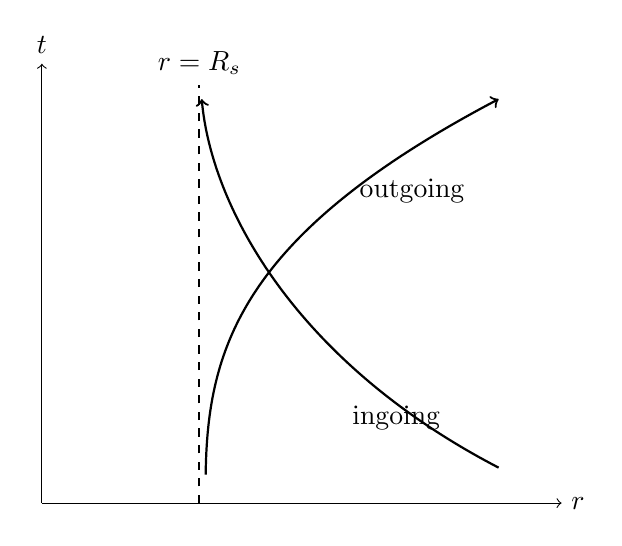
\begin{tikzpicture}[x=1.0cm,y=0.9cm]
\draw[->] (0,0) -- (6.6,0) node[right] {$r$};
\draw[->] (0,0) -- (0,6.2) node[above] {$t$};
\draw[dashed,thick] (2.0,0) -- (2.0,5.9) node[above] {$r=R_s$};
\draw[thick,->] (2.08,.4) .. controls (2.10,2.2) and (2.55,3.8) .. (5.8,5.7);
\draw[thick,->] (5.8,.5) .. controls (3.2,2.0) and (2.15,4.2) .. (2.03,5.7);
\node[align=center] at (4.7,4.4) {outgoing};
\node[align=center] at (4.5,1.2) {ingoing};
\end{tikzpicture}
\caption{Phiên bản theo thời gian tọa độ đã được làm gọn của bản phác thảo trên bảng. Sự chậm lại biểu kiến là một phát biểu về \(t\) trong tọa độ Schwarzschild, không phải về việc ánh sáng cục bộ không còn chuyển động với \(c\).}
\end{figure}

Bên trong chân trời, các nón ánh sáng tương lai nghiêng vào trong đến mức cả hai nhánh theo phương bán kính hướng về tương lai đều dẫn tới \(r\) giảm. Không tín hiệu nào phát sinh ở đó có thể thoát ra ngoài, và mọi đường nhân quả hướng về tương lai đều đi tới kỳ dị.

\begin{classroomqa}
\audiencequestion{Nếu tốc độ ánh sáng là bất biến, thì nói chính xác là gì khi bảo rằng ánh sáng chậm lại gần chân trời?\lecturetimestamp{00:31:44}}
\lecturerresponse{Đại lượng được hiển thị là \(dr/dt\) trong một hệ tọa độ cụ thể. Tốc độ dưới dạng giá trị số đã thay đổi khi mét được thay bằng xentimét; ở đây các chuẩn hiệu dụng theo phương bán kính và theo thời gian còn biến thiên theo vị trí. Mệnh đề phổ quát là mọi tia sáng đều đi theo một quỹ đạo null, \(ds^2=0\).}
\end{classroomqa}
\editorialnote{Một quan sát viên cục bộ rơi tự do đo ánh sáng trong chân không là \(c\); việc vận tốc theo tọa độ Schwarzschild triệt tiêu ở chân trời không phải là một đại lượng quan sát cục bộ.}

\begin{classroomqa}
\audiencequestion{Mệnh đề về tốc độ null ấy có còn đúng bất kể ánh sáng truyền qua môi trường vật chất nào hay không?\lecturetimestamp{00:33:24}}
\lecturerresponse{Không. Tư liệu hiện có không còn lưu phần giải thích dài hơn cho câu trả lời này.}
\end{classroomqa}
\editorialnote{Khẳng định về tốc độ null nói về sự lan truyền trong không-thời gian chân không. Tương tác với vật chất có thể khiến một gói sóng có tốc độ hiệu dụng nhỏ hơn; đó là tính chất của môi trường, không phải sự thay đổi của tốc độ nhân quả cục bộ \(c\).}

\begin{classroomqa}
\audiencequestion{Một tia sáng đi vào trông như thế nào trên cùng giản đồ \(t\)-\(r\)?\lecturetimestamp{00:33:32}}
\lecturerresponse{Đó là nhánh có hình dạng ngược lại: từ \(r\) lớn, nó uốn về phía chân trời và tiến tới đó một cách tiệm cận. Nó cần một lượng thời gian tọa độ \(t\) vô hạn để tới nơi.}
\end{classroomqa}
\editorialnote{Một quan sát viên rơi vào tới chân trời và đi qua nó trong thời gian riêng hữu hạn; chỉ có \(t\) Schwarzschild là phân kỳ.}

\section{Vì sao sự bay hơi tạo ra một vấn đề}

Chân trời còn đáng được nghiên cứu nhiều hơn nữa: nó hình thành ra sao, người quan sát rơi vào thấy gì, và liệu ở đó có điều gì bất thường về cục bộ hay không. Susskind hoãn các câu hỏi ấy lại và chuyển thẳng sang cơ học lượng tử. Từ bên ngoài nhìn vào, vật chất cùng toàn bộ thông tin phân biệt của nó bị nén ngày càng sát chân trời hơn và trở nên không thể tiếp cận. Chỉ riêng điều đó chưa nhất thiết hủy diệt thông tin; có thể nó chỉ đơn giản là che giấu thông tin.

Kết quả của Hawking làm vấn đề trở nên gay gắt. Một lỗ đen cổ điển đã ổn định trông như vật thể tẻ nhạt nhất có thể tưởng tượng: có đối xứng cầu, tối, và không thể gửi đi một thông điệp. Nhưng ``đen'' có hai nghĩa. Nó có thể có nghĩa là không phát ra gì cả, hoặc có thể có nghĩa là phát bức xạ nhiệt vật đen. Một lỗ đen lượng tử là đen theo nghĩa thứ hai. Nó có nhiệt độ, phát sáng và mất năng lượng. Vì
\begin{equation}
E=Mc^2,
\qquad
R_s=\frac{2GM}{c^2},
\end{equation}
bức xạ làm giảm cả khối lượng lẫn bán kính chân trời của nó. Nếu sự bay hơi cuối cùng làm lỗ đen biến mất, thì thông tin dường như vẫn còn ở chân trời của nó sẽ ra sao? Nó có thể bị hủy, bị giữ lại trong một tàn dư tí hon, hoặc được mã hóa trong bức xạ đi ra. Sự căng thẳng giữa những khả năng đó chính là bài toán thông tin, và về sau lý thuyết dây sẽ giúp làm sắc nét cách giải quyết nó.

Tối nay không thử thực hiện phép tính nào về trường lượng tử trong không-thời gian cong. Thay vào đó, Susskind đi theo con đường đơn giản hơn của Bekenstein: trước hết hiểu entropy như thông tin, rồi tính xem lỗ đen có thể che giấu bao nhiêu thông tin.

\section{Thông tin hiện diện nhưng bị che giấu}

Hãy tưởng tượng chia một chiếc hộp thành những ô đủ nhỏ sao cho mỗi ô hoặc có vật chiếm chỗ hoặc trống. Một chuỗi nhị phân---mỗi ô một câu trả lời---phân biệt cấu hình đó với mọi cấu hình được phép khác. Vật chất thực tế hơn đòi hỏi các câu hỏi về loại hạt và những bậc tự do khác, nhưng nguyên lý không đổi: thông tin được đo bằng số tối thiểu các câu hỏi có--không cần để xác định trạng thái.

\begin{classroomqa}
\audiencequestion{Đây có phải chỉ là mô tả của một hệ tĩnh không?\lecturetimestamp{00:45:49}}
\lecturerresponse{Đó là mô tả tức thời, tại một thời điểm. Khi đó động lực học ánh xạ trạng thái ấy sang một trạng thái khác.}
\end{classroomqa}

Nguyên lý tiếp theo còn sâu hơn: sự tiến hóa của một hệ kín không gộp hai trạng thái vi mô khác nhau thành một. Nếu hai cấu hình khác nhau ở hiện tại, thì các cấu hình đã tiến hóa của chúng về nguyên tắc vẫn còn phân biệt được. Sự tiến hóa Hamilton cổ điển là khả nghịch và sự tiến hóa lượng tử là đơn nhất.\editorialnote{Các phương trình hiệu dụng tiêu tán chỉ có thể xóa những khác biệt ấy vì các bậc tự do môi trường không được quan sát đã bị bỏ qua; trạng thái kín đầy đủ vẫn giữ chúng.}

Ví dụ bồn tắm làm cho sự khác nhau giữa mất mát và không thể tiếp cận trở nên cụ thể. Hai dòng giọt nước có thể mã hóa hai thông điệp Morse khác nhau. Sau khi nước lắng xuống, cả hai bồn trông như nhau. Các gợn sóng nhìn thấy được đã biến mất, nhưng một phép đo vi mô đầy đủ vẫn sẽ tìm thấy các cấu hình phân tử khác nhau. Thông điệp đã lan ra các bậc tự do quá nhỏ và quá nhiều để theo dõi.

Entropy chính là thông tin bị che giấu này. So với những câu hỏi vĩ mô mà ta có thể đặt---nhiệt độ, năng lượng toàn phần, thành phần, mực nước---nhiều phân biệt vi mô vẫn có thể tồn tại nhưng không thể tiếp cận. Theo ngôn ngữ đếm bit của bài giảng,
\begin{equation}
S=\hbox{number of hidden bits}.
\end{equation}
Công thức thống kê chính xác là \(S=k_B\ln\Omega\), nhưng định nghĩa định tính là đủ cho lập luận về lỗ đen.

\section{Nhiệt độ như cái giá phải trả để che giấu một bit}

Nhiệt độ là đại lượng quen thuộc để đo nhưng lại được định nghĩa một cách gián tiếp đến đáng ngạc nhiên. Susskind chọn entropy và năng lượng làm các khái niệm nguyên thủy. Giả sử một bit máy tính được đặt lại về một giá trị chuẩn. Thiết bị vật lý vẫn còn đó, nhưng sự phân biệt giữa các trạng thái 0 và 1 trước đây của nó biến mất khỏi máy tính. Nó không thể biến mất khỏi thế giới đầy đủ; nó được chuyển sang các bậc tự do vi mô trong môi trường, khiến môi trường nóng lên một chút. Đây là nguyên lý Landauer.

Nếu lấy một đơn vị entropy là một bit và đo nhiệt độ theo đơn vị năng lượng, thì trong bài giảng viết
\begin{align}
\Delta S&=1,\\
\Delta E&=T\,\Delta S,\\
dE&=T\,dS.
\label{eq:first-law}
\end{align}

\begin{figure}[htbp]
\centering
\includegraphics[width=0.84\textwidth]{lecture_02_figure_04.png}
\caption{Nhiệt động lực học theo lý thuyết thông tin trên bảng: \(S\) là entropy, một bit bị ẩn có \(\Delta S=1\), và chi phí năng lượng tối thiểu của nó được viết là \(\Delta E=T\Delta S\).}
\lectureframe{00:58:40.000}
\end{figure}

\editorialnote{Trong các đơn vị thông thường, chi phí xóa thuận nghịch của một bit nhị phân là \(k_BT\ln2\). Phương trình~\eqref{eq:first-law} dùng \(k_B=1\) và coi đơn vị entropy của bài giảng là một bit đồng thời lược bỏ \(\ln2\) đi kèm. Các quy ước này không ảnh hưởng đến lập luận theo bậc độ lớn ở phần sau.}

Một ước tính từ cử tọa đặt độ tăng nhiệt độ tối thiểu của một cốc nước do xóa khoảng \(100\) gigabyte ở vào cỡ \(10^{-15}\) độ. Susskind chấp nhận ý chính chứ không chấp nhận con số chính xác: ở nhiệt độ phòng, một bit mang một năng lượng tối thiểu cực kỳ nhỏ, và máy tính thực tỏa nhiệt nhiều hơn rất nhiều vì việc xóa không được thực hiện một cách thuận nghịch.

\begin{classroomqa}
\audiencequestion{Ví dụ về ổ cứng chỉ là một phép loại suy, hay sự nung nóng do xóa là một định luật thực sự?\lecturetimestamp{01:00:02}}
\lecturerresponse{Đó là một ràng buộc vật lý thực sự, nguyên lý Landauer. Việc đặt lại một ô nhớ loại bỏ sự phân biệt cũ khỏi máy tính, nên thông tin ấy phải được mang ra môi trường. Các thao tác thông thường kém hiệu quả hơn mức tối thiểu lý tưởng rất nhiều vì chúng còn phải vận hành mạch, di chuyển điện tích và tạo ra nhiệt không liên quan.}
\end{classroomqa}

\begin{classroomqa}
\audiencequestion{Ẩn một bit ở nhiệt độ cao hơn có tốn nhiều năng lượng hơn không?\lecturetimestamp{01:02:07}}
\lecturerresponse{Có. Hệ thức \(dE=T\,dS\) nói đúng như vậy: với cùng một lượng entropy được truyền đi, một bể nhiệt nóng hơn đòi hỏi một lượng năng lượng truyền lớn hơn. Cũng có thể xem quan hệ năng lượng trên mỗi bit bị ẩn này như là định nghĩa của nhiệt độ.}
\end{classroomqa}

\begin{classroomqa}
\audiencequestion{Nếu ta ghi đè lên một bit đã lưu trước đó, thì thông tin cũ ấy có bị mất không?\lecturetimestamp{01:02:43}}
\lecturerresponse{Nó đã rời khỏi máy tính, nhưng không biến mất khỏi hệ vật lý kín. Sự phân biệt bị ghi đè ấy đã bị phân tán vào môi trường, nơi nó góp phần tạo nên thông tin không thể tiếp cận và vì thế là entropy.}
\end{classroomqa}

Việc đồng nhất entropy nhiệt động học với thông tin vi mô bị thiếu đã có từ Boltzmann; Shannon đã cung cấp ngôn ngữ lý thuyết thông tin tương ứng trong thế kỷ XX. Susskind nhận xét rằng lời giải thích này đã vắng mặt một cách kỳ lạ trong các khóa học nhiệt động lực học mà ông và các thành viên cử tọa từng học vào những năm 1950. Khoa học máy tính khiến mối liên hệ ấy khó bị bỏ qua hơn, nhưng không khởi nguyên nội dung vật lý của nó.

\section{Đưa một bit vào một lỗ đen}

Giờ đây ta có thể xây dựng một lỗ đen về mặt khái niệm, từng bit một, giống như có thể đổ đầy bồn tắm từng giọt. Câu hỏi mang tính vi phân: khi thêm một bit bị ẩn nữa, chân trời tăng lên bao nhiêu? Hãy bắt đầu với một lỗ đen có khối lượng \(M\) và bán kính \(R_s\), rồi đưa vào vật đơn giản nhất mà sự phân biệt duy nhất còn có thể phục hồi được là nó có bị hấp thụ hay không.

\begin{classroomqa}
\audiencequestion{Chẳng phải thông tin cần thời gian tọa độ vô hạn để đi vào lỗ đen sao?\lecturetimestamp{01:08:07}}
\lecturerresponse{Nó bị nén theo hàm mũ gần chân trời và trở nên không còn khả dụng đối với bên ngoài chỉ sau một thời gian thực tế ngắn, dù thời gian tọa độ Schwarzschild gán cho việc thực sự đi qua một giá trị vô hạn. Vì vậy, trong cách hạch toán từ bên ngoài, có thể coi nó như được lưu tại chân trời.}
\end{classroomqa}

Photon là một ứng viên tự nhiên, nhưng một photon tổng quát mang nhiều hơn một bit. Phân cực của nó có thể mã hóa một lựa chọn nhị phân. Một điểm đi vào được định xứ rất sắc nét đem lại thêm nhiều câu hỏi có--không nữa: bán cầu trên hay dưới, nửa trái hay phải, v.v. Cơ học lượng tử giới hạn việc định xứ vào cỡ một bước sóng, nên cách triệt bớt thông tin vị trí là dùng bước sóng dài nhất mà lỗ đen vẫn còn hấp thụ được.

\begin{classroomqa}
\audiencequestion{Có thật sự có một bước sóng cực đại mà vượt quá nó thì photon không thể đi vào không?\lecturetimestamp{01:12:15}}
\lecturerresponse{Có. Một sóng lớn hơn lỗ đen rất nhiều chủ yếu bị tán xạ chứ không bị hấp thụ. Lựa chọn biên hữu ích là bước sóng so sánh được với bán kính chân trời: đủ dài để xóa mờ điểm đi vào, nhưng vẫn đủ ngắn để có xác suất hấp thụ đáng kể.}
\end{classroomqa}

\begin{classroomqa}
\audiencequestion{Bản thân hướng mà photon đi tới có làm tăng thêm thông tin không?\lecturetimestamp{01:13:28}}
\lecturerresponse{Với bước sóng cỡ toàn bộ chân trời, trường biến thiên chậm đến mức trên phạm vi lỗ đen nên không thể phân giải hướng tới với độ chính xác cao. Đây là lý do giới hạn bước sóng dài được xấp xỉ bằng một dữ kiện có--không duy nhất, thay vì một cú va chạm được định vị sắc nét.}
\end{classroomqa}

Vì vậy, xét theo bậc độ lớn, chọn
\begin{equation}
\lambda\sim R_s=\frac{2GM}{c^2}.
\label{eq:one-bit-wave}
\end{equation}
Động học của photon cho
\begin{equation}
E=cp,
\qquad
p=\hbar k=\frac{h}{\lambda},
\qquad
\Delta E\sim\frac{\hbar c}{R_s}.
\label{eq:one-bit-energy}
\end{equation}
Ở đây \(k=2\pi/\lambda\) và \(h=2\pi\hbar\). Bài giảng cố ý bỏ qua \(2\pi\), cũng như các hệ số hấp thụ cỡ đơn vị.

\begin{classroomqa}
\audiencequestion{Động lượng nên viết là \(\hbar/\lambda\), hay \(h/\lambda\)?\lecturetimestamp{01:16:00}}
\lecturerresponse{Với \(\lambda\) là bước sóng thông thường, hệ thức chính xác là \(p=h/\lambda=2\pi\hbar/\lambda\); còn với số sóng \(k=2\pi/\lambda\) thì là \(p=\hbar k\). Trong ước lượng hiện tại chỉ giữ lại bậc độ lớn, nên hệ số \(2\pi\) được cố ý bỏ đi.}
\end{classroomqa}

Chi phí năng lượng để ẩn một bit chính là thang nhiệt độ. Vì vậy, các phương trình~\eqref{eq:one-bit-wave} và~\eqref{eq:one-bit-energy} cho
\begin{equation}
k_BT_H\sim\frac{\hbar c}{R_s}
\sim\frac{\hbar c^3}{GM}.
\end{equation}
Kết quả chính xác của Hawking là
\begin{equation}
k_BT_H=\frac{\hbar c^3}{8\pi GM}.
\end{equation}
Lập luận sơ cấp cho đúng sự phụ thuộc vào \(M,G,c,\hbar\), nhưng không cho đúng hệ số.

\section{Một bit chiếm một mảnh diện tích cỡ Planck}

Photon ấy cũng cho ta biết chân trời tăng như thế nào. Năng lượng của nó làm khối lượng thay đổi một lượng
\begin{equation}
\Delta M=\frac{\Delta E}{c^2}
\sim\frac{\hbar}{cR_s}.
\end{equation}
Vì \(R_s=2GM/c^2\),
\begin{equation}
\Delta R_s=\frac{2G}{c^2}\Delta M
\sim\frac{G\hbar}{c^3R_s},
\end{equation}
trong đó mọi hệ số cỡ đơn vị lại một lần nữa đều bị lược bỏ. Nhân với \(R_s\),
\begin{equation}
R_s\Delta R_s\sim\frac{G\hbar}{c^3}.
\end{equation}
Vì \(A=4\pi R_s^2\), vi phân của nó là \(dA=8\pi R_s\,dR_s\). Do đó
\begin{equation}
\Delta A\sim\frac{G\hbar}{c^3}=\ell_P^2,
\qquad
\ell_P=\sqrt{\frac{G\hbar}{c^3}}.
\label{eq:planck-patch}
\end{equation}

\begin{figure}[htbp]
\centering
\includegraphics[width=0.84\textwidth]{lecture_02_figure_05.png}
\caption{Lập luận theo bậc độ lớn hoàn chỉnh trên bảng: năng lượng của một bit \(\Delta E\sim\hbar c/R_s\) dẫn đến độ tăng của bình phương bán kính, và do đó của diện tích, ở cỡ \(G\hbar/c^3\).}
\lectureframe{01:22:40.000}
\end{figure}

Trong phép tính trực tiếp, các thừa số \(c\) được khôi phục ở giữa chừng và một người trong cử tọa phát hiện \(c^{-2}\) bị thiếu trong bán kính Schwarzschild. Chính hiệu chỉnh đó tạo ra \(c^{-3}\) trong Phương trình~\eqref{eq:planck-patch}.

\begin{classroomqa}
\audiencequestion{Việc chỉ khôi phục \(c\) trong một phần phép tính có làm mất hai lũy thừa của nó không?\lecturetimestamp{01:21:18}}
\lecturerresponse{Có. Hệ thức đúng về thứ nguyên là \(R_s=2GM/c^2\), chứ không đơn giản là \(2GM\). Khôi phục thừa số ấy làm cho thang diện tích trở thành \(G\hbar/c^3\).}
\end{classroomqa}

Dùng \(G\simeq6.7\times10^{-11}\,\mathrm{m^3\,kg^{-1}\,s^{-2}}\), \(\hbar\simeq1.05\times10^{-34}\,\mathrm{J\,s}\) và \(c^3\simeq2.7\times10^{25}\,\mathrm{m^3\,s^{-3}}\),
\begin{equation}
\ell_P^2\simeq2.6\times10^{-70}\,\mathrm{m^2},
\qquad
\ell_P\simeq1.6\times10^{-35}\,\mathrm{m}.
\end{equation}
Trong khi thực hiện ước lượng trên bảng, các số mũ được nói ra trong bài giảng có lúc chệch đi; kết luận vật lý thì vẫn ổn định. Thang này nhỏ hơn rất xa độ phân giải thực nghiệm trực tiếp.

Hình ảnh dễ nhớ là những bit không thể xuyên qua nhau, với những khuỷu tay nhọn, tích tụ trên chân trời và đẩy nhau sang bên. Mỗi bit mới chiếm xấp xỉ một mảnh diện tích Planck. Đó là một ẩn dụ cho việc hạch toán theo diện tích, không phải là khẳng định rằng chân trời thực sự được ghép từ những ô vuông.

\begin{classroomqa}
\audiencequestion{Nếu photon thứ nhất vẫn còn đang tiến đến khi một photon khác làm chân trời nở ra, thì chẳng phải photon cũ sẽ nằm bên trong chân trời mới sao?\lecturetimestamp{01:26:39}}
\lecturerresponse{Bức tranh tĩnh đơn giản không đủ chính xác để phân định câu hỏi đó. Chân trời sự kiện trong một không-thời gian động phải được định nghĩa toàn cục, và vị trí của nó thay đổi khi vật chất đi tới. Trong mô tả từ bên ngoài được dùng ở đây, thông tin vẫn gắn với chân trời đang lớn dần. Một định nghĩa cẩn thận về chân trời ấy được để lại cho sau.}
\end{classroomqa}

\begin{classroomqa}
\audiencequestion{Vấn đề ấy có nảy sinh tương tự khi thêm vào một khối lượng rất lớn, chẳng hạn khi hai lỗ đen va chạm, không?\lecturetimestamp{01:27:03}}
\lecturerresponse{Có; khi đó không thể bỏ qua tính động của bài toán. Bài giảng hoãn việc bàn hình học đầy đủ của sự sáp nhập cho đến khi chân trời được định nghĩa cẩn thận hơn.}
\end{classroomqa}

\begin{classroomqa}
\audiencequestion{Diện tích Planck chỉ được định nghĩa trên một mảnh phẳng, thay vì trên một chân trời hình cầu, phải không?\lecturetimestamp{01:27:30}}
\lecturerresponse{Nó là một thang diện tích trên bề mặt cầu, chứ không phải yêu cầu chân trời phải phẳng. Sự phân biệt phẳng hay cầu không có ý nghĩa đáng kể đối với phép đếm này.}
\end{classroomqa}
\editorialnote{Khi bán kính độ cong của chân trời lớn hơn \(\ell_P\) rất nhiều, mỗi lân cận cỡ Planck đều gần như phẳng cục bộ.}

Đối với một lỗ đen có bề ngang tám kilômét, photon ở ngưỡng tương ứng sẽ là một sóng vô tuyến dài có cỡ xấp xỉ như thế. Một phép loại suy từ cử tọa so sánh độ tăng diện tích không phụ thuộc kích thước với việc thêm cùng một phần chu vi vào một sợi dây quấn quanh quả bóng rổ hoặc quanh Trái Đất: trong mỗi trường hợp, khoảng hở theo bán kính được tạo ra bởi cùng một phần chu vi tăng thêm là như nhau. Hình học chính xác của hai trường hợp là khác nhau, nhưng cả hai ví dụ đều cô lập một độ biến thiên không phụ thuộc vào kích thước ban đầu của vật thể.

\section{Định luật diện tích}

Việc thêm từng bit một làm thay đổi diện tích chân trời một lượng vi mô phổ quát. Vì vậy, số bit có thể bị ẩn phải tỉ lệ với \(A/\ell_P^2\), chứ không phải với thể tích. Bekenstein suy ra tính tỉ lệ ấy; phép tính của Hawking cố định hệ số của nó:
\begin{equation}
S_{\mathrm{BH}}=\frac{k_B A c^3}{4G\hbar}
=\frac{k_B A}{4\ell_P^2}.
\label{eq:bh-entropy}
\end{equation}
Nếu entropy được đếm bằng bit nhị phân thay vì đơn vị nhiệt động học, hãy chia \(S_{\mathrm{BH}}/k_B\) cho \(\ln2\).

\begin{figure}[htbp]
\centering
\includegraphics[width=0.84\textwidth]{lecture_02_figure_06.png}
\caption{Công thức cuối cùng trên bảng, kể cả hệ số \(1/4\) của Hawking: \(S\propto Ac^3/(4G\hbar)\) theo đơn vị entropy dùng trong bài giảng.}
\lectureframe{01:31:02.000}
\end{figure}

Vì thế, lỗ đen có entropy lớn hơn các hệ thông thường có kích thước tương đương, với một khoảng cách khổng lồ. Tuy nhiên, đáp án vẫn nhỏ hơn điều mà một phép đếm theo thể tích một cách ngây thơ có thể gợi ý. Lượng thông tin độc lập bị chặn bởi một đại lượng bề mặt. Sự đảo ngược này---một vùng hấp dẫn ba chiều được mô tả bằng thông tin tỉ lệ theo một biên hai chiều---là mầm mống của nguyên lý toàn ảnh.

\begin{classroomqa}
\audiencequestion{Hệ số \(1/4\) trong công thức entropy từ đâu mà ra?\lecturetimestamp{01:30:30}}
\lecturerresponse{Lập luận của Bekenstein xác định sự phụ thuộc vào diện tích và các hằng số cơ bản nhưng để lại một hệ số chưa biết; các ước lượng của ông cho ra những khả năng như logarit của hai. Phép tính trường lượng tử của Hawking cố định hệ số ấy chính xác bằng \(1/4\).}
\end{classroomqa}

Vị trí của \(\hbar\) chứa đựng bất ngờ cuối cùng. Người ta có thể nghĩ rằng một entropy lượng tử sẽ tỉ lệ với \(\hbar\) và triệt tiêu trong giới hạn cổ điển. Thay vào đó, \(\hbar\) lại nằm ở mẫu số. Khi \(\hbar\to0\), một sóng có thể mang thông tin tinh vi tùy ý với chi phí năng lượng nhỏ tùy ý, nên dung lượng entropy phân kỳ. Sự lượng tử hóa không cộng thêm một entropy nhỏ vào một lỗ đen vốn dĩ cổ điển; nó ngăn không cho khả năng chứa thông tin trở nên vô hạn.

\begin{classroomqa}
\audiencequestion{Vì sao \(\hbar\), có đơn vị là mômen động lượng, lại cũng xác lập quan hệ giữa động lượng thông thường và bước sóng?\lecturetimestamp{01:33:23}}
\lecturerresponse{\(\hbar\) có đơn vị của tác dụng, tương đương với động lượng nhân khoảng cách. Vì \(p\lambda\) có cùng đơn vị ấy, nên quan hệ lượng tử có thể là \(p\sim\hbar/\lambda\), tùy theo quy ước \(2\pi\). Mômen động lượng \(\mathbf r\times\mathbf p\) có cùng thứ nguyên vì cùng một lý do.}
\end{classroomqa}

Bài giảng dừng ở đây, không phải vì chủ đề đã cạn mà vì đây là ranh giới thích hợp. Hình học đã cho ta biết vì sao chân trời che giấu thông tin; nhiệt động lực học đã cho ta biết cách đếm thông tin bị che giấu; cơ học lượng tử đã cung cấp một diện tích hữu hạn cho mỗi bit. Câu hỏi tiếp theo không còn là liệu lỗ đen có các trạng thái vi mô hay không, mà là những trạng thái ấy mã hóa và rốt cuộc trả lại những gì đã rơi vào như thế nào.
